\chapter*{Niveau 4}
\addcontentsline{toc}{chapter}{Niveau 4}
Det siges, at guderne skabte verden ved at bringe lys og mørke sammen. Du gør det samme, når du bringer det mørke stål til den lyse flamme. I din smedje er du en gud, og stål og panser bøjer sig for din vilje og du har det sidste ord.\\


\begin{tabular}{|p{0.705\textwidth}|p{0.2350\textwidth}|}
\hline
\rowcolor{cerulean!80}
 \multicolumn{2}{|c|}{ Mestersmed } \\
\hline
\rowcolor{cerulean!40}
    Evne navn & Pris i XP\\ \hline
    Ekstra NK Niv. 4 & 1\\\hline
    Hellig smed & 3 \\\hline
    Læse/Skrive Hellig  & 1\\\hline
    Låse Mekaniker & 2 \\\hline
    Perfektionist & 3 \\\hline
    Runesmedning   & 4\\\hline
\end{tabular}

\section*{Evne beskrivelse for Mestersmed}
\addcontentsline{toc}{section}{Evne beskrivelse for Mestersmed}

\subsection*{Ekstra NK Niv. 4}
\addcontentsline{toc}{subsection}{Ekstra NK Niv. 4}
Du har et ekstra nævekamp.\\

\subsection*{Hellig smed}
Du skal vælge en gud, hvis du ikke allerede har gjort dette. Når du smeder på denne guds hellig grund vil det tage halvt så lang tid. Dette inkludere at reparer rustning, lave låse og smede rune genstande.\\
Har din gud ikke en aktiv hellig grund, bedes du kontakte en arrangør for at udrede dette.

\input{mainstuff/Evner/Læse og skrive Hellig}

\subsection*{Låse Mekaniker}
Låse du laver vil springe i luften når de bliver dirket op. Du skal markere din lås med et blåt bånd udover det normale bånd du bruger. Hvis nogen dirker denne lås vil de tage skade. Skaden vil være det dobbelte af låsens niveau.\\
Husk at gøre opmærksom på dette når du sælger låsen. Hvis den sættes på en kiste bør kisten indeholde en note hvor på denne effekt står.\\
For at bruge denne evne skal du bruge sulfur når du laver en lås. Mængden af sulfur du skal bruge er det dobbelt af låsens niveau. Når den er sprunget i luften en gang, vil låsen stadig være på plads, men vil ikke sprænge igen før du har sat nyt sulfur i den af en smed.


\subsection*{Perfektionist}
\addcontentsline{toc}{subsection}{Perfektionist}
En Mestersmed kan få det bedste ud af de ressourcer personen har til rådighed. Derfor kan de fremstille produkter med mindre materiale. Når en perfektionist bruger jern til at lave genstande så som låse, ovs, så skal de kun bruge halvt så meget jern, rundet op.\\

En mestersmed er også i stand til at kombinere 5 jern og 5 manakrystaller for at skabe 1 mitril. Dette tager 10 minutter. Dette ødelægger både jern og manakrystaller. Dette bliver ikke reduceret.\\


\subsection*{Runesmedning}
\addcontentsline{toc}{subsection}{Runesmedning}
\textbf{For at tage denne evne skal du have Læse og Skrive Hellig.}\\
Det første du skal vide om runer er, at de \emph{IKKE} er magiske. Runer er en opfindelse af dværgene, som blev lavet for at bekæmpe magi og magiske væsner. Derfor er runer altså anti-magiske genstande og de kan derfor aldrig fortrylles.\\
Det tager 5 minutter per ingrediens at smede en rune genstand.\\
Runegenstande har dog nogle overnaturlige kræfter, som gør at de bliver bundet til den sjæl som bærer dem. Dette betyder at en rune genstand ikke kan stjæles, men ejeren kan frit give sin rune genstand til en anden person. Den, der modtager en rune genstand som gave vil blive den nye ejer, og rune genstanden kan nu ikke tages fra dem. En usmedet rune kan dog stadig stjæles.\\

En færdig smedet runegenstand markeres ved et hvidt bånd, hvorpå runens navn er skrevet med sort. Dette bånd skal altid sidde på runegenstanden. Mangler båndet har runegenstanden ingen effekt, før du skaffer et nyt bånd at sætte på. Runesmeden har selv ansvaret for at skaffe de off-game materialer, der skal bruges til at markere en runegenstand.\\

\textbf{At bruge runegenstande}\\
Du kan bruge forskellige runegenstande på samme tid, der findes dog visse begrænsninger. Du kan
kun eje 1 runevåben, 1 runerustning og 1 runeskjold af gangen, altså én af hver type.\\
Du kan f.eks. ikke eje runer i flere forskellige dele af din rustning, ligesom du ikke kan bruge og bærer 2 runevåben på samme tid.\\

Magikastere (inklusiv præster) kan ikke bære og benytte runegenstande.\\

Runesmeden er i stand til at omsmede runer. Det vil sige at han kan forme en type rune til en anden. Dette tager 10 minutter. Hvis du har en assistent til at hjælpe dig tager det 5 minutter.\footnote{Vi foreslår kraftigt at bruge en yngre spiller.}\\
\textit{F.eks.\\Bjarne har en Nagerune, men han skal bruge en Jernrune. Han giver derfor sin Nagerune til en RuneSmed som omdanner hans Nagerune til en Jernrune.}\\

\textbf{Nagerune}\\
Denne rune siges at være den ældste rune, der eksisterer. Dens kræfter bruges med offensivt henblik. Dette var også den første rune, som thanen Even Ûhr Krezz opdagede, da han fandt runernes kraft dybt i sit folks bjerge.\\
\begin{figure}[H]
    \centering
    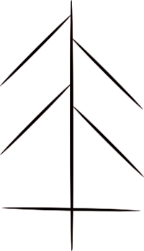
\includegraphics[height=5.5cm]{setup/Pictures/Nagerune.png}
    \caption{Nagerune}
\end{figure}

\textbf{Elementrune}\\
Denne rune besidder alle elementernes kræfter. Hvordan den er opstået ved ingen præcist, men dværgene har dog legender, der fortæller om et uhyre, som levede i fortiden som skabte denne rune. Elementrunens kræfter kan være både offensive og defensive.\\
\begin{figure}[H]
    \centering
    
\includegraphics[height=5.5cm]{setup/Pictures/Elementrune.png}
    \caption{Elementrune}
\end{figure}

\textbf{Jernrune}\\
Denne rune er skabt til beskyttelse. Ifølge legenden blev den skabt af thanen Altika, som levede generationen efter Even Ûhr Krezz. Til tider er denne rune også kendt for at have
helbredende egenskaber.
\begin{figure}[H]
    \centering
    
\includegraphics[height=5.5cm]{setup/Pictures/Jernrune.png}
    \caption{Jernrune}
\end{figure}

\textbf{Dragerune}\\
Den nyeste rune, som først lige er blevet magtfuld. Med ophøjelsen af Esselia og dragernes Opvågning, har denne rune nu fået ny magt, som forstyrrer balancen.\\
\begin{figure}[H]
    \centering
    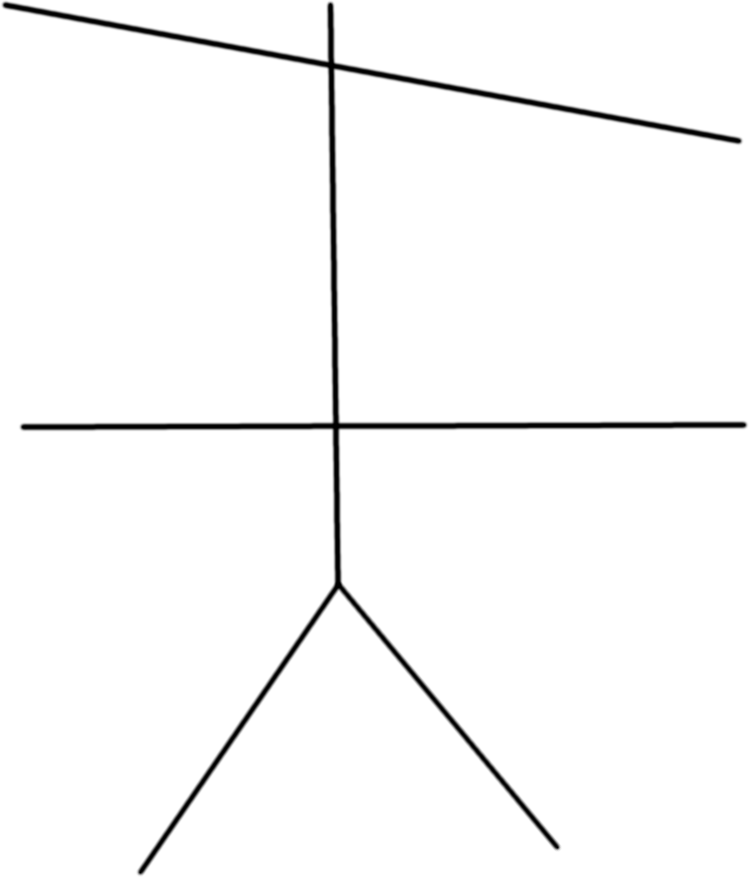
\includegraphics[height=5.5cm]{setup/Pictures/Dragerune.png}
    \caption{Dragerune}
\end{figure}

\begin{runeskjold*}[Drageskind]
\textbf{Effekt:} Du tager kun halvt så meget skade fra magier. (rundet op)\\
\textbf{Ingredienser:} 3 Elementruner, 3 Drageruner, 2 Jernruner.
\end{runeskjold*}

\begin{runeskjold*}[Essalias beskyttelse]
\textbf{Effekt:} Du får dobbelt så meget liv når du bliver helbredt.\\
\textbf{Ingredienser:} : 1 Elementrune, 1 Dragerune.
\end{runeskjold*}

\begin{runeskjold*}[Krigerens Skjold]
\textbf{Effekt:} Dette skjold giver dig 1 RP på samme måde som en normal rustningsdel vil. Det ekstra RP fra dit skjold vil altid være det første du mister; dette ekstra RP mistes kun når du selv rammes og ikke når nogen slår på skjoldet. Dette RP kan repareres som normalt hos en smed.\\
\textbf{Ingredienser:} : 1 Jernrune.
\end{runeskjold*}

\begin{runeskjold*}[Magiens Bane]
\textbf{Effekt:} Dette runeskjold gør bæreren i stand til 2 gange per døgn, at modstå en valgfri magi som rammer spilleren. Når spilleren rammes af en magi, de vil beskyttes imod, skal de udtale kommandoen: ”Magiens Bane – immun!”\\
\textbf{Ingredienser:} 4 Jern, 2 Jernruner, 2 Elementruner, 1 Dragerune.
\end{runeskjold*}

\begin{runevåben*}[Armens styrke]
\textbf{Effekt:} Bæreren af dette våben vil modtage 5 ekstra NK så længe de har våbenet på sig.\\
\textbf{Ingredienser:} 1 Nagerune
\end{runevåben*}

\begin{runevåben*}[Heksejægeren]
\textbf{Effekt:} En gang per døgn kan du ophæve en magi, hvis du rammer en person eller barriere med dette våben. Du kan ikke ophæve magiske genstande, såsom talismaner med dette våben.\\
\textbf{Ingredienser:} 1 Jern, 1 Sjælestøv, 1 Nagerune, 1 Jernrune, 1 Elementrune, 1 Dragerune.
\end{runevåben*}

\begin{runevåben*}[Kellwans Klinge]
\textbf{Effekt:} Dette våben giver permanent hellig skade. Dette skal som normalt markeres med et grønt bånd. (For optimal effekt kan dette også siges ved slag på fjender, hvor hellig skade kan have effekt.)\\
\textbf{Ingredienser:} 1 Nagerrune, 1 Elementrune.
\end{runevåben*}

\begin{runevåben*}[Livets Le]
\textbf{Effekt:} Når du dræber en person med dette våben vil du genvinde 1 mistet LP. Du kan ikke gå over din maksimale LP ved brug af dette våben.\\
\textbf{Ingredienser:} 1 Flagermuse gødning, 1 Elementrune, 2 Nagerruner, 1 Dragerune
\end{runevåben*}

\begin{runevåben*}[Magerens Mareridt]
Dette våben har ingen effekt i kamp. Det kan bruges til tortur, hvor den vil syge vilje og fokus fra ethvert offer. Tortureres en person med mana i kroppen, vil de miste mana i stedet for LP, med samme interval på 1 mana per minut. Offerets mana kan først genvindes 1 time efter torturen er afsluttet. Har offeret ingen mana (tilbage) i kroppen, vil de miste LP som ved normal tortur.
Note: Denne rune genstand tæller ikke mod det samlet antal rune genstande du må have på dig. Denne rune kan sættes på alle torturinstrumenter.\\
\textbf{Ingredienser:} 1 Nagerrune, 1 Enhjørningeblod.
\end{runevåben*}

\begin{runerustning*}[Dragens Rustning]
\textbf{Effekt:} 2 gange pr. scenarie kan du ved at berøre nogen bruge kommandoen: ”Drageild – 6 hellig skade”. Du vælger selv hvornår du bruger kommandoen.\\
\textbf{Ingredienser:} 4 Sulfur, 2 Dragerune, 2 Elementrune, 1 Ildgræs.
\end{runerustning*}

\begin{runerustning*}[Gudernes Rustning]
\textbf{Effekt:} Negative magier påvirker dig nu kun halvt så lang tid (rundet op.)\\
\textbf{Ingredienser:} 3 Drageruner, 1 Elementrune.
\end{runerustning*}

\begin{runerustning*}[Hærførens Rustning]
\textbf{Effekt:} Denne rustning giver dig 3 ekstra RP. Disse RP fungerer på samme måde som de normale RP du får fra en normal rustning. De ekstra RP vil altid være det første, du mister og de sidste der, bliver repareret.\\
\textbf{Ingredienser:} 4 Jern, 3 Jernruner.
\end{runerustning*}

\begin{runerustning*}[Jordens Rustning]
\textbf{Effekt:} Du bliver immun overfor alle vælte effekter\\
\textbf{Ingredienser:} 2 Jernruner, 2 Elementruner, 1 Flagermuse gødning.
\end{runerustning*}

\begin{runerustning*}[Krigerens Rustning]
\textbf{Effekt:} Denne rustning giver dig 2 ekstra RP. Disse RP fungerer på samme måde som de normale RP du får fra en normal rustning. De ekstra RP vil altid være det første, du mister og de sidste der, bliver repareret.\\
\textbf{Ingredienser:} 2 jern, 1 Jernrune.
\end{runerustning*}

\begin{runerustning*}[Samaritanernes Rustning]
\textbf{Effekt:} Hvis du går på 0 LP mens du bærer denne rustning, vil du automatisk genvinde alle dine naturlige LP 10 minutter efter du vågner; dvs. når du igen er kampdygtig ifølge dødsreglerne, som findes i det almindelige regelsæt.\\
\textbf{Ingredienser:} 1 Jernrune, 1 Enhjørningeblod.
\end{runerustning*}

\begin{runerustning*}[Thanens Rustning]
\textbf{Effekt:} Denne rustning reparerer alt din udrustning på mystisk vis. Dette betyder, at du genvinder 1 RP pr. 2. minut når du bærer rustningen og er ved bevidsthed. Du kan ikke genvinde mere RP end du normalt får for din rustning.\\
\textbf{Ingredienser:} 1 Jernrune, 1 Elementrune.
\end{runerustning*}